\documentclass{standalone}
\usepackage[OT1]{fontenc}
\renewcommand*\familydefault{\sfdefault}
\usepackage{helvet,sfmath}
\usepackage{tikz}
\begin{document}



\tikzset{every picture/.style={line width=0.75pt}} %set default line width to 0.75pt        

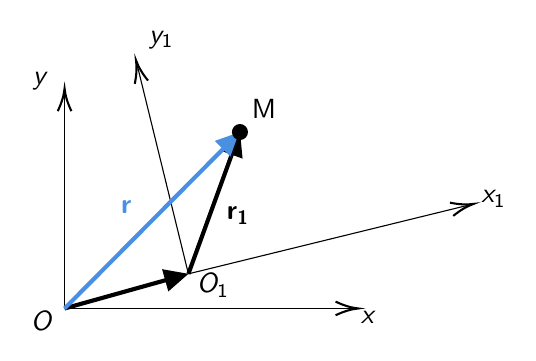
\begin{tikzpicture}[x=0.75pt,y=0.75pt,yscale=-1,xscale=1]
%uncomment if require: \path (0,15225); %set diagram left start at 0, and has height of 15225

%Straight Lines [id:da1856418731209697] 
\draw    (836,910) -- (975.5,910) ;
\draw [shift={(977.5,910)}, rotate = 180] [color={rgb, 255:red, 0; green, 0; blue, 0 }  ][line width=0.75]    (10.93,-3.29) .. controls (6.95,-1.4) and (3.31,-0.3) .. (0,0) .. controls (3.31,0.3) and (6.95,1.4) .. (10.93,3.29)   ;
%Straight Lines [id:da5915919331589892] 
\draw    (836,910) -- (836,806) ;
\draw [shift={(836,804)}, rotate = 90] [color={rgb, 255:red, 0; green, 0; blue, 0 }  ][line width=0.75]    (10.93,-3.29) .. controls (6.95,-1.4) and (3.31,-0.3) .. (0,0) .. controls (3.31,0.3) and (6.95,1.4) .. (10.93,3.29)   ;
%Straight Lines [id:da8503307333016918] 
\draw [line width=1.5]    (836,910) -- (891.81,894.4) ;
\draw [shift={(895.66,893.33)}, rotate = 164.39] [fill={rgb, 255:red, 0; green, 0; blue, 0 }  ][line width=0.08]  [draw opacity=0] (11.61,-5.58) -- (0,0) -- (11.61,5.58) -- cycle    ;
%Straight Lines [id:da5372268061515848] 
\draw    (895.66,893.33) -- (1031.15,860.1) ;
\draw [shift={(1033.09,859.62)}, rotate = 166.22] [color={rgb, 255:red, 0; green, 0; blue, 0 }  ][line width=0.75]    (10.93,-3.29) .. controls (6.95,-1.4) and (3.31,-0.3) .. (0,0) .. controls (3.31,0.3) and (6.95,1.4) .. (10.93,3.29)   ;
%Straight Lines [id:da8084979884763777] 
\draw    (895.66,893.33) -- (870.89,792.32) ;
\draw [shift={(870.41,790.38)}, rotate = 76.22] [color={rgb, 255:red, 0; green, 0; blue, 0 }  ][line width=0.75]    (10.93,-3.29) .. controls (6.95,-1.4) and (3.31,-0.3) .. (0,0) .. controls (3.31,0.3) and (6.95,1.4) .. (10.93,3.29)   ;
%Straight Lines [id:da8560201744429087] 
\draw [line width=1.5]    (895.66,893.33) -- (919.13,828.76) ;
\draw [shift={(920.5,825)}, rotate = 109.98] [fill={rgb, 255:red, 0; green, 0; blue, 0 }  ][line width=0.08]  [draw opacity=0] (11.61,-5.58) -- (0,0) -- (11.61,5.58) -- cycle    ;
%Straight Lines [id:da10202852418593888] 
\draw [color={rgb, 255:red, 74; green, 144; blue, 226 }  ,draw opacity=1 ][line width=1.5]    (836,910) -- (917.68,827.84) ;
\draw [shift={(920.5,825)}, rotate = 134.83] [fill={rgb, 255:red, 74; green, 144; blue, 226 }  ,fill opacity=1 ][line width=0.08]  [draw opacity=0] (11.61,-5.58) -- (0,0) -- (11.61,5.58) -- cycle    ;
%Straight Lines [id:da7241429536854683] 
\draw    (920.5,825) -- (895.66,893.33) ;
\draw [shift={(920.5,825)}, rotate = 109.98] [color={rgb, 255:red, 0; green, 0; blue, 0 }  ][fill={rgb, 255:red, 0; green, 0; blue, 0 }  ][line width=0.75]      (0, 0) circle [x radius= 3.35, y radius= 3.35]   ;

% Text Node
\draw (819.5,795) node [anchor=north west][inner sep=0.75pt]   [align=left] {$\displaystyle y$};
% Text Node
\draw (977.5,910) node [anchor=north west][inner sep=0.75pt]   [align=left] {$\displaystyle x$};
% Text Node
\draw (818.5,910) node [anchor=north west][inner sep=0.75pt]   [align=left] {$\displaystyle O$};
% Text Node
\draw (898.5,892) node [anchor=north west][inner sep=0.75pt]   [align=left] {$\displaystyle O_{1}$};
% Text Node
\draw (1035.5,852) node [anchor=north west][inner sep=0.75pt]   [align=left] {$\displaystyle x_{1}$};
% Text Node
\draw (875.5,775) node [anchor=north west][inner sep=0.75pt]   [align=left] {$\displaystyle y_{1}$};
% Text Node
\draw (862,857) node [anchor=north west][inner sep=0.75pt]    {$\mathbf{\textcolor[rgb]{0.29,0.56,0.89}{r}}$};
% Text Node
\draw (913,860) node [anchor=north west][inner sep=0.75pt]    {$\mathbf{r_{1}}$};
% Text Node
\draw (925,820) node [anchor=south west] [inner sep=0.75pt]   [align=left] {M};


\end{tikzpicture}
\end{document}